
\begin{sidewaysfigure}[p]
    \centering
    \begin{subfigure}[b]{0.45\textwidth}
        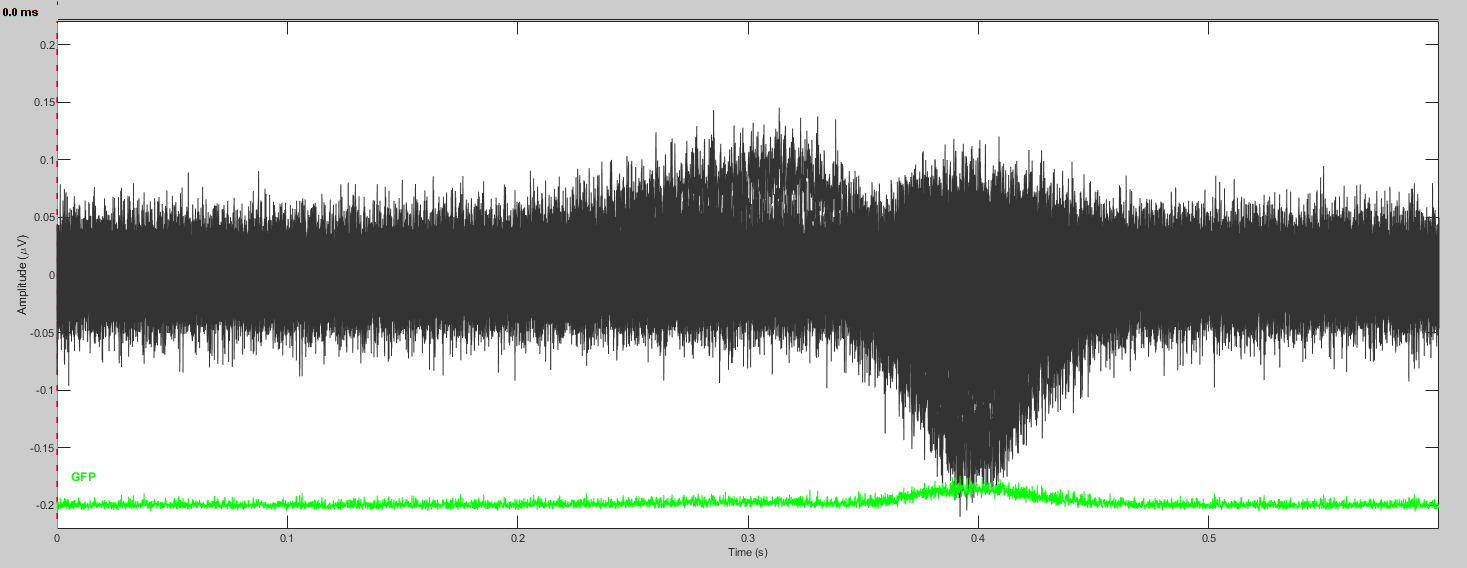
\includegraphics[width=\textwidth]{eeg/eeg-d1n1c9c9.png}
        \caption{Señales de EEG simuladas con BSCR 20.}
        \label{fig:eeg-d1n1c9c9}
        \vspace{1em}
    \end{subfigure}
    \hfill
    \begin{subfigure}[b]{0.45\textwidth}
        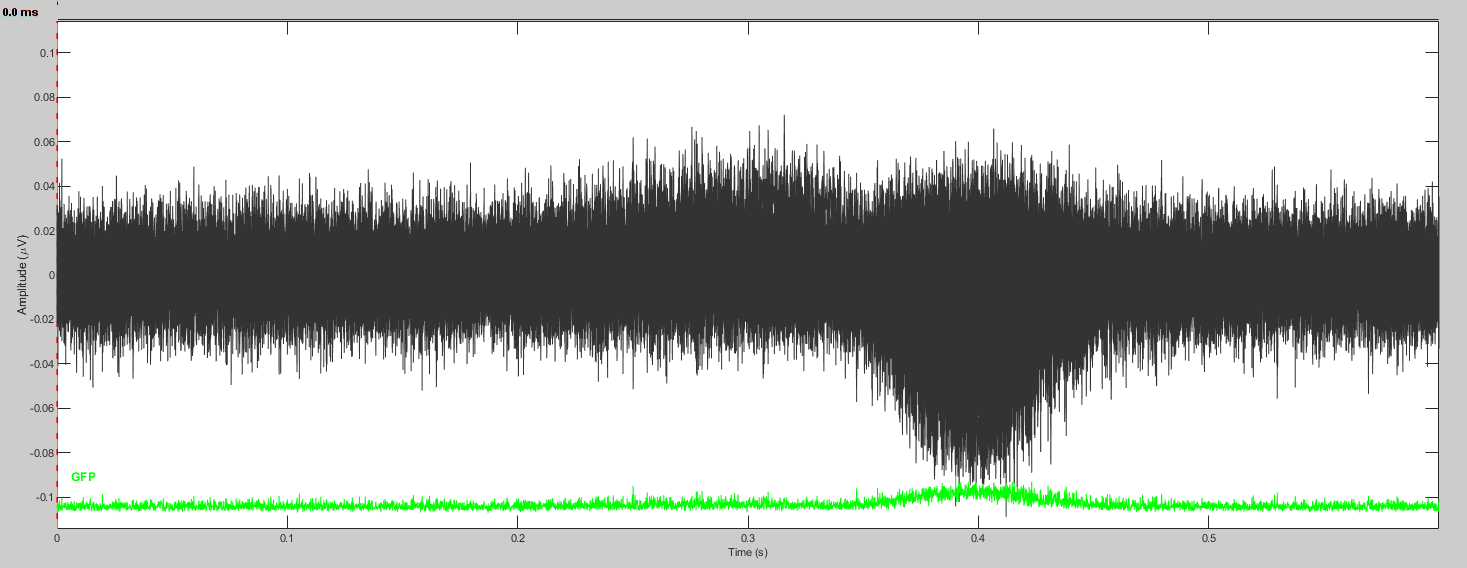
\includegraphics[width=\textwidth]{eeg/eeg-d1n1c10c10.png}
        \caption{Señales de EEG simuladas con BSCR 80.}
        \label{fig:eeg-d1n1c10c10}
        \vspace{1em}
    \end{subfigure}
    \vfill
    \begin{subfigure}[b]{0.45\textwidth}
        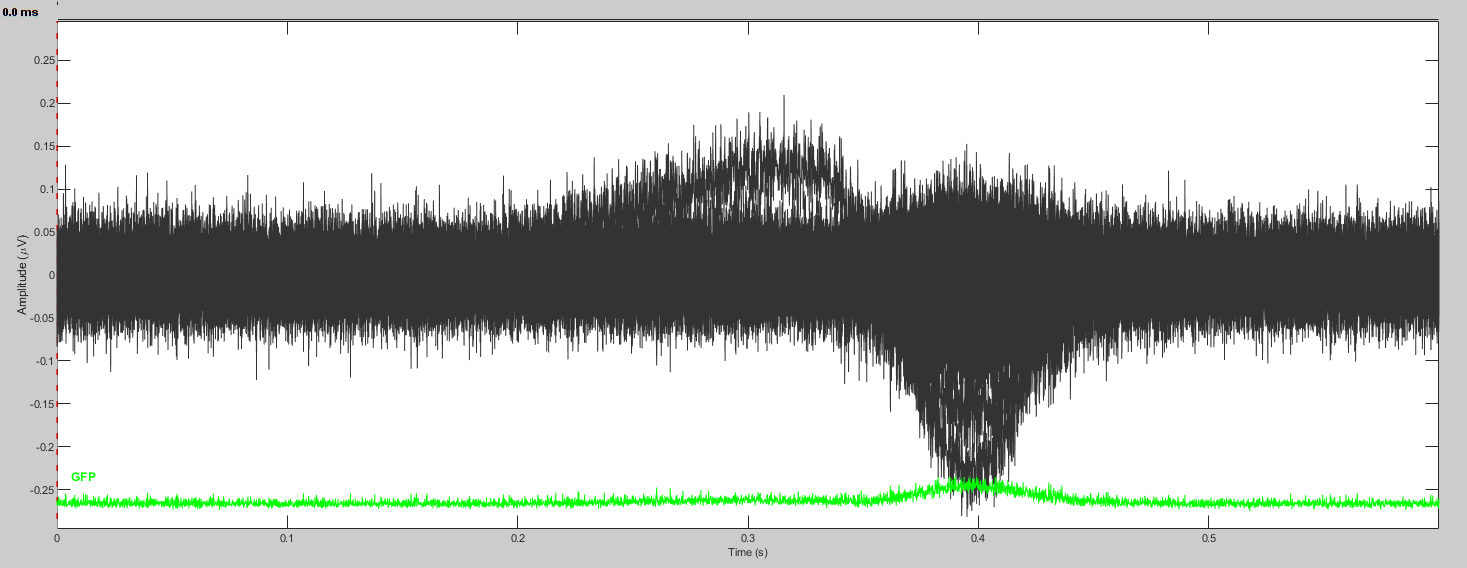
\includegraphics[width=\textwidth]{eeg/eeg-d1n1c8c8.png}
        \caption{Señales de EEG simuladas con BSCR 10.}
        \label{fig:eeg-d1n1c8c8}
    \end{subfigure}
    \hfill
    \begin{subfigure}[b]{0.45\textwidth}
        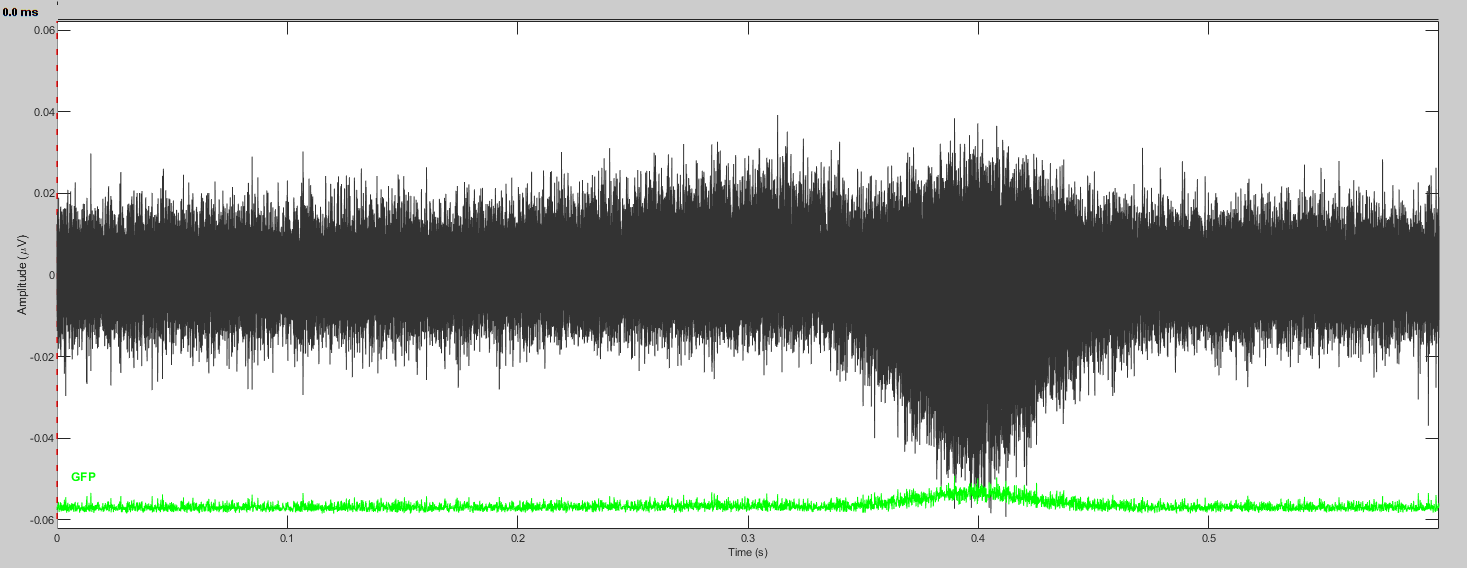
\includegraphics[width=\textwidth]{eeg/eeg-d1n1c2c2.png}
        \caption{Señales de EEG simuladas con BSCR 200.}
        \label{fig:eeg-d1n1c2c2}
    \end{subfigure}
    \caption{Señales de EEG simuladas con diferentes valores de BSCR.}
    \label{fig:eeg-simulated}
\end{sidewaysfigure}